% !TEX root = ../discriminative_filtering.tex

\section{Introduction}
Supervised training methods are often classified by their underlying probabilistic model.  For inputs $x$ and outputs $y$ , generative methods learn the joint distribution $p(x,y)$, discriminative methods learn the conditional distribution $p(y|x)$, and algorithmic methods learn the decision boundary directly.  

%%%%%%%%%%%%%%%%%%%%%%%%%%%%%%%%%%%%%%%%%%%%%%%%%
\section{Nadaraya--Watson Kernel Regression} \index{Nadaraya-Watson kernel regression}
Given a dataset $\{(x_i,z_i)\}_{i=1}^n$, we can use Kernel Density Estimation (KDE) to model the joint density:
\[
p(z,x) \approx \frac{1}{n} \sum_{i=1}^n \kappa_Z(z,Z_i)\kappa_X(x,X_i).
\]
where  $\kappa_Z(z,z')$ and $\kappa_X(x,x')$ are kernel functions (symmetric, positive-definite).  It follows that the conditional distribution is then given by
\begin{equation} \label{e:kde_condl}
p(z|x) 
= \frac{p(z,x)}{p(x)} 
\approx \frac{\sum_{i=1}^m \kappa_Z(z,Z_i)\kappa_X(x,X_i)}{ \sum_{i=1}^m \kappa_X(x,X_i)}.
\end{equation}
We then estimate $f(x):=\mathbb{E}[Z|X=x]$ as
\begin{equation}
  f(x) = \int z p(z|x) dz \approx  \frac{\sum_{i=1}^m \left(\int z \kappa_Z(z,Z_i) dz\right) \kappa_X(x,X_i)}{ \sum_{i=1}^m \kappa_X(x,X_i)}  
\end{equation}
Because the kernel is symmetric, $\int z \kappa_Z(z,z') dz = z'$ so that 
\begin{equation} \label{e:NW_f}
f(x) \approx  \frac{\sum_{i=1}^m Z_i \kappa_X(x,X_i)}{ \sum_{i=1}^m \kappa_X(x,X_i)}
\end{equation}
This is the well-known Nadaraya-Watson kernel regression estimator~\cite{Nad64, Wat64}.  In the same vein, we may estimate
\begin{equation}
    \mathbb{E}[Z^\intercal Z|X=x]\approx  \frac{\sum_{i=1}^m \left(\int z^\intercal z \kappa_Z(z,Z_i) dz\right) \kappa_X(x,X_i)}{ \sum_{i=1}^m \kappa_X(x,X_i)}
\end{equation}
If the kernel is both symmetric and stationary, so that $\int z^\intercal z \kappa_Z(z,z') dz = \Sigma_Z + (z')^\intercal z'$ for some fixed $\Sigma_Z\in \mathbb{S}_d$, then
\begin{equation} \label{e:NW_x2}
\mathbb{E}[Z^\intercal Z|X=x]\approx  \Sigma_Z + \frac{\sum_{i=1}^m Z_i^\intercal Z_i \kappa_X(x,X_i)}{ \sum_{i=1}^m \kappa_X(x,X_i)}
\end{equation}
If Equations~\ref{e:NW_f} and~\ref{e:NW_x2} hold, we can then form an estimate for $Q(x):=\var[ Z|X=x]$ as follows
\begin{equation} \label{e:NW_Q}
Q(x) \approx \Sigma_Z + \frac{\sum_{i=1}^m Z_i^\intercal Z_i \kappa_X(x,X_i)}{ \sum_{i=1}^m \kappa_X(x,X_i)} - (f(x))^\intercal f(x)
\end{equation}

%%%%%%%%%%%%%%%%%%%%%%%%%%%%%%%%%%%%%%%%%%%%%%%%%
\begin{figure}[h]
\begin{minipage}[c]{.35\textwidth}
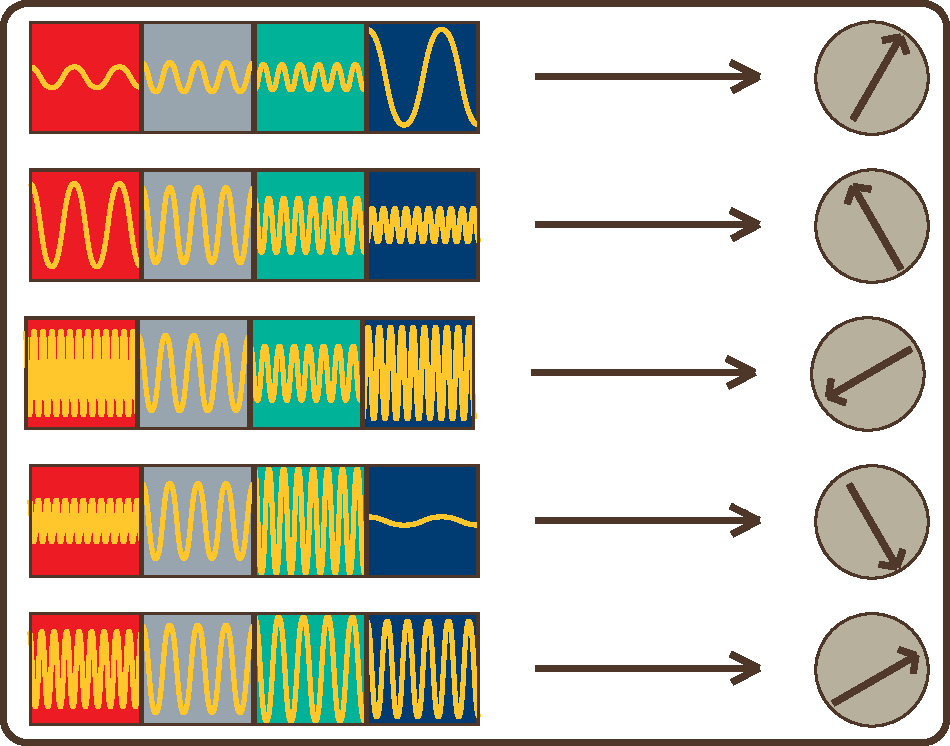
\includegraphics[width=\linewidth]{nw_dataset}
\end{minipage}%
\hfill
\begin{minipage}[c]{.55\textwidth}
\caption[Nadaraya--Watson Kernel Regression]{The Nadaraya--Watson kernel regression estimate takes a training dataset $\mathcal{D}$ (left) and for a testpoint $x_*$ returns (up to renormalization) an estimate for the corresponding $z_*$-value that is the weighted sum of the training values, where the weights for each $z_i$ are determined by how close the corresponding $x_i$ is to $x_*$ (as determined by the kernel):
}
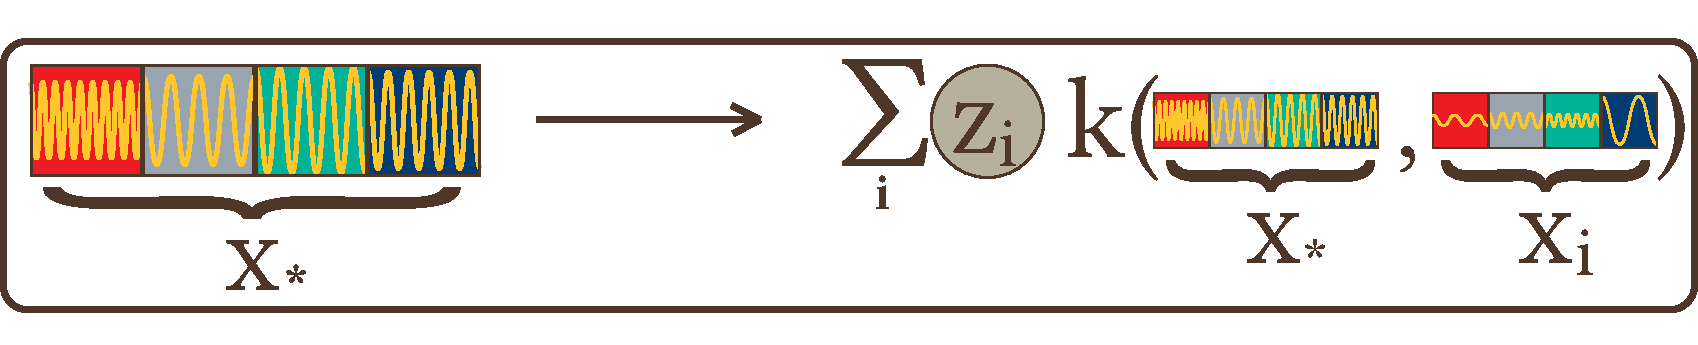
\includegraphics[width=\linewidth]{nw_inference}
\end{minipage}
\end{figure}

\subsection{Learning}
Learning kernel bandwidth parameters can be done via cross-validation or a rule of thumb (e.g. Silverman's rule).

%%%%%%%%%%%%%%%%%%%%%%%%%%%%%%%%%%%%%%%%%%%%%%%%%
\section{Neural Network Regression with Homoskedastic Gaussian Noise} \index{neural networks!for nonlinear regression}
Given a dataset $\{(x_i,y_i)\}_{i=1}^n$, we can model
\begin{equation}
    Y_i = f(X_i) + \epsilon_i
\end{equation}
where $\epsilon_i\sim^\text{i.i.d.}\N(\vec 0, \Gamma)$ and $f$ is some unknown nonlinear function.  We can learn $f$ from training data  as a neural network.  The idea is to form f by recursively composing a nonlinear activation function $a$ with linear combinations of inputs
\begin{align}
    f_1(x) &= a(L_0x) \\ 
    f_2(x) &= a(L_1f_1(x)) \\
    &\vdots \\
    f_m(x) &= L_m a(L_{m-1}f_{m-1}(x))
\end{align}
where at each step, the input is first multiplied by some matrix $L_i$ and then the function $a$ is applied to each coordinate of the output.  

\subsection{Learning}
Training a neural network then corresponds to solving the optimization problem:
\begin{equation}
    \hat L_0,\dotsc,\hat L_m = \argmin_{L_0,\dotsc,L_m} \norm{Y_{1:n} - f_m(X_{1:n})}
\end{equation}
Any functional relationship can be approximated arbitrarily well (if $m\ge 1$, i.e. if there is at least one hidden layer) by the above approach as the size of $L_0,L_1$ become arbitrarily large; this is known as the Universal Approximation Theorem~\cite{Hor91}.

\subsection{Issues and Innovations}
Choosing the architecture; i.e. the sizes for the $L_i$ (sizes of the hidden layers) and the nature of the activation functions (max-pooling, dropout, convolution, batch normalization) is amazingly challenging and oftentimes done painstakingly by hand~\cite{Rea17,Zop17}.

%%%%%%%%%%%%%%%%%%%%%%%%%%%%%%%%%%%%%%%%%%%%%%%%%
\section{Gaussian Process Regression} \index{Gaussian process regression}
Given a dataset $\{(x_i,y_i)\}_{i=1}^n$, a Gaussian process regression models the random variables $Y_i$ as joint Gaussian with covariance 
\begin{equation} \label{e:gp_cov}
    \cov(Y_i,Y_j) = \kappa_\theta(x_i,x_j)
\end{equation}
where $\kappa$ is a kernel function (symmetric, positive-definite) dependent on a set $\theta$ of tunable hyperparameters.  The model is then
\begin{equation}\label{e:gp_full}
    \begin{bmatrix} Y_{1:n} \\ Y_* \end{bmatrix}
    \sim \N\left( \vec 0, \begin{bmatrix} \kappa_\theta(x_{1:n},x_{1:n}) & \kappa_\theta(x_{1:n},x_*) \\ \kappa_\theta(x_*,x_{1:n}) &  \kappa_\theta(x_*,x_*) \end{bmatrix} \right)
\end{equation}
where $(x_*,Y_*)$ denotes the random value of $Y_*$ at a deterministic point $x_*$.  We let  $K := \kappa_\theta(x_{1:n},x_{1:n})$ denote the matrix given by $K_{ij} = \kappa_\theta(x_i,x_j)$.  Under this notation, we have also $K_*:= \kappa_\theta(x_{1:n},x_*)$ and $K_{**} := \kappa_\theta(x_*,x_*)$, so we may re-write \eqref{e:gp_full} as
\begin{equation}\label{e:gp_abbrev}
    \begin{bmatrix} Y_{1:n} \\ Y_* \end{bmatrix}
    \sim \N\left( \vec 0, \begin{bmatrix} K & K_* \\ K_*^\intercal &  K_** \end{bmatrix} \right)
\end{equation}
This implies
\begin{equation} \label{e:gp_inf}
    Y_*|x_{1:n},Y_{1:n}, x_*
    \sim \N(K_*^\intercal K^{-1} Y_{1:n}, K_{**} - K_*^\intercal K^{-1} K_*)
\end{equation}
When the model specifies noisy observations, so that \eqref{e:gp_cov} becomes
\begin{equation} \label{e:gp_cov_noisey}
    \cov(Y_i,Y_j) = \kappa_\theta(x_i,x_j) + \sigma^2 \delta_{\{i=j\}}
\end{equation}
the inference \eqref{e:gp_inf} becomes
\begin{equation} \label{e:gp_inf_noisey}
    Y_*|x_{1:n},Y_{1:n}, x_*
    \sim \N(K_*^\intercal (K+\sigma^2 I)^{-1} Y_{1:n}, K_{**} - K_*^\intercal (K+\sigma^2 I)^{-1} K_*)
\end{equation}
where $I=I_n$ denotes the $n$-dimensional identity matrix.  It's worth noting that the mean function for a Gaussian process is a linear combination of kernel functions, i.e.
\begin{equation}
    \Exp[Y_*|x_{1:n},Y_{1:n}, x_*] = \sum_{i=1}^n \alpha_i \kappa_\theta(x_i,x_*)
\end{equation}
where $\alpha =(K+\sigma^2 I)^{-1} Y_{1:n}$.

%%%%%%%%%%%%%%%%%%%%%%%%%%%%%%%%%%%%%%%%%%%%%%%%%
\begin{figure}[h]
\begin{minipage}[t]{.45\textwidth}
\begin{center}
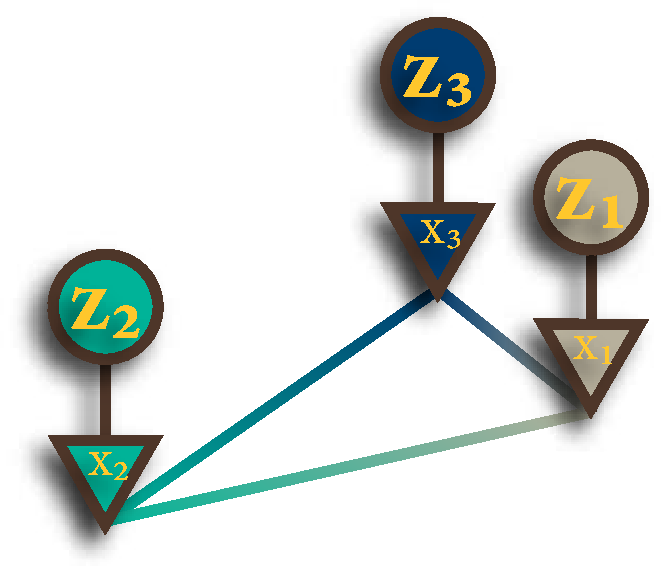
\includegraphics[width=0.8\linewidth]{gp_model}
\end{center}
\caption[Gaussian Process Model]{GP model. Given a dataset ${\mathcal{D} = \{(x_i,z_i)\}_{i=1}^n}$, the GP model specifies that \\
$\begin{bmatrix} z_1 \\ z_2 \\ z_3 \end{bmatrix} 
\sim \N\left(\begin{bmatrix} 0 \\ 0 \\ 0 \end{bmatrix}, \begin{bmatrix} k_{11} & k_{12} & k_{13} \\ k_{21} & k_{22} & k_{23} \\ k_{31} & k_{32} & k_{33} \end{bmatrix} + \sigma^2 I \right)$
where $k_{ij} = k_\theta(x_i,x_j)$ and $\sigma^2$ accounts for noisy measurements.  The model specifies that more similar $x$-values (as determined by the kernel) should correspond to more correlated $z$-values.
}
\end{minipage}%
\hfill
\begin{minipage}[t]{.45\textwidth}
\begin{center}
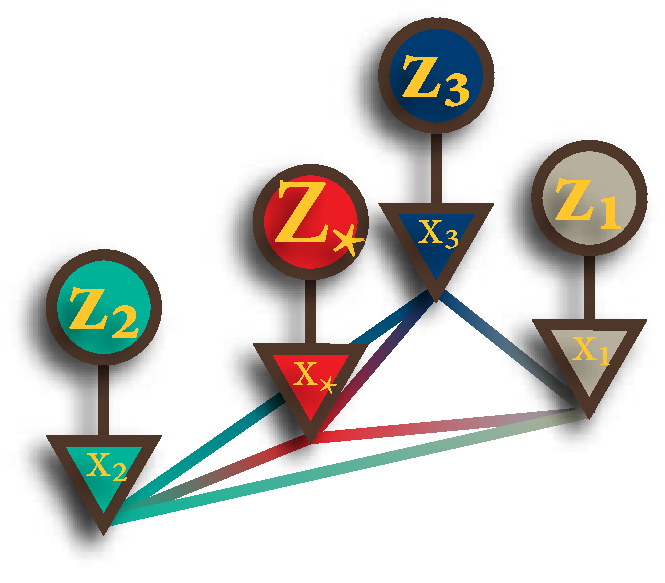
\includegraphics[width=0.8\linewidth]{gp_inference}
\end{center}
\caption[Gaussian Process Inference]{GP Inference. Given some test value $x_*$, we now have\\
$ \begin{bmatrix} \top \\ z \\ \bot \\ \textcolor{red}{Z_*} \end{bmatrix} 
\sim \N\left(\begin{bmatrix} \top \\ 0 \\ \bot \\ \textcolor{red}{0} \end{bmatrix}, \begin{bmatrix} \ulcorner &  & \urcorner & \textcolor{red}{\top} \\  \multicolumn{3}{c}{K+\sigma^2 I}   & \textcolor{red}{k_*} \\ \llcorner &  & \lrcorner &  \textcolor{red}{\bot} \\ \textcolor{red}{\vdash} & \textcolor{red}{k_{*}^\tr} & \textcolor{red}{\dashv} &  \textcolor{red}{k_{**}} \end{bmatrix} \right).$
From this, $Z_*|\{X_*=x_*, \mathcal{D}\}$ can be calculated.  This is the prediction given in \eqref{e:gp_inf}.
}
\end{minipage}
\end{figure}

\subsection{Learning}
To learn the model \eqref{e:gp_inf_noisey} (which reduces to \eqref{e:gp_inf} when $\sigma^2=0$), we usually consider the log-likelihood of the data
\begin{equation}
    \log p(Y_{1:n}|x_{1:n}) = -\frac{1}{2} Y_{1:n}^\intercal (K+\sigma^2 I)^{-1} Y_{1:n} - \frac{1}{2} \log\abs{K + \sigma^2 I} - \frac{n}{2} \log 2\pi
\end{equation}
The most common method of choosing hypeparameters is by maximizing the MLE:
\begin{equation}
    \hat\theta_{MLE}, \hat\sigma_{MLE} = \argmax_{\theta,\sigma} \log p(Y_{1:n}|x_{1:n})
\end{equation}
where the dependence on $\theta$ occurs through the matrix $K$.  See \cite{Ras06} for other hyperparameter learning methods.

\subsection{Issues and Innovations}
GP prediction scales $\mathcal{O}(n^3)$ in computational cost with the size of the training set because the full covariance matrix $K$ must be inverted.  The issue of requiring the entire training dataset in order to perform prediction proves a particular downside to nonparametric models, including GP's.  (We can contrast this to, e.g. linear regression, where the learned coefficients are sufficient for prediction.)  To this end, some researchers asked \emph{could one replace the original training set with a much smaller (optimized) pseudo-training set, with only minimal alteration to the predictions?}  From the different ways to measure alteration and perform optimization arise a family of methods known collectively as sparse Gaussian processes~\cite{Qui05}.  \index{Gaussian process regression!sparse} The optimized pseudo-training points are variously referred to as pseudo-inputs, inducing points, or support points.  It's possible the sparse GP's may provide other incidental benefits with respect to robustness: \cite{Sne05} remarked that \begin{quote} although the [sparse GP] is not specifically designed to model nonstationarity, the extra flexibility associated with moving pseudo-inputs around can actually achieve this to a certain extent. \end{quote}


%%%%%%%%%%%%%%%%%%%%%%%%%%%%%%%%%%%%%%%%%%%%%%%%%
\section{Random Forests} \index{random forest}
We can also approximate $p(z_t|x_t)$ as a random forest, one type of ensemble method.  The idea behind ensemble methods is to agglomerate a set of weak learners (learners that may be only slightly better than chance) into a strong learner (one that becomes arbitrarily good as the number of its constituents grows).  In the case of random forests, the weak learner is a regression tree.  A regression tree partitions the $x_t$ space and assigns a constant value to each of the partition members.  
\begin{equation}
f_j(x) = \sum_{i=1}^{N_j} c^j_i \mathds{1}_{C^j_i}(x)
\end{equation}
Numerous algorithms exist to optimize these choices.  A regression forest then combines many of these trees $f_1,\dotsc, f_T$ into a single estimator.  Under the model for $Z|X$ that first draws a tree randomly from $\{1,\dotsc,T\}$ and then assigns the estimate from that tree, we have the model
\begin{equation}
    p(z|x) = 
    \begin{cases} 1/N_j, & z=c_{\{i: x\in C_i^j\}}^j \\
    0, & \text{otherwise}
    \end{cases}
\end{equation}
Under this model it follows that
\begin{equation}
    \Exp[Z|X=x] = \frac{1}{N_j} \sum_{j=1}^{N_j} c_{\{i: x\in C_i^j\}}^j = \frac{1}{N_j} \sum_{j=1}^{N_j} f_j(x)
\end{equation}
and
\begin{equation}
    \Exp[ZZ^\intercal|X=x] = \frac{1}{N_j} \sum_{j=1}^{N_j} f_j(x)( f_j(x))^\intercal
\end{equation}

